% Thesis introduction
% Author: Tore.
%

In this chapter the background information needed in order to understand the topics of this thesis and its papers is given. First, in Section \ref{sec:gpgpu}, general-purpose programming on graphics processing units (\nom{GPGPU}{General-purpose programming on graphics processing units}) is reviewed, followed by an introduction to medical ultrasound imaging in Section \ref{sec:ultrasound}. Finally, the concepts of volume rendering and field simulations are presented in Section \ref{sec:volren} and \ref{sec:field}.

\section{General-purpose computing on graphics processing units}\label{sec:gpgpu}
In a recent essay, Herb Sutter, a leading authority on software development, reviews the current state of the software and computer industry \cite{HerbSutter}. The essay bears the name "Welcome to the Jungle" and is a sequel to the essay "The Free Lunch is Over" from 2004 \cite{HerbSuttera}. The two essays spins around the fact that chip manufactures hit a frequency-wall in the beginning of the 21st century. Until then, all mainstream computer programs where typically running in a single thread on a single core, and a programmer could expect the software to annually gain performance without touching the code. This was the "free-lunch" era as depicted in Fig.\,\ref{fig:jungle}. The increase in processing power came mostly from an ever-growing clock frequency. However, power consumption and heat generation where also growing at the same rate, until the level of cooling required finally became to much in 2004.  From that point, chip manufactures had to pursue a different approach  than just increasing the clock frequency. The immediate solution was to embed several cores in one CPU chip. This insured continuation of Moore's law, since the number of transistors per chip could continue to grow. For programmers, multi-core CPUs meant that computer programs now had to be multi-threaded in order to continue to gain performance. It was a concurrency revolution, and  the free lunch was over.

\begin{figure}
\centering
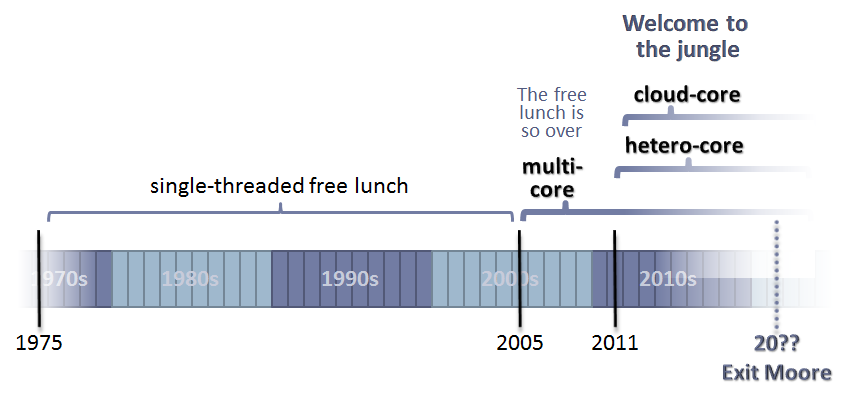
\includegraphics[width=0.9\textwidth]{img/free_lunsh.png}
\caption{Illustration of several transitions currently taking place in the computer industry. \todo{Site Herb Sutter - Welcom to the jungle http://herbsutter.com/welcome-to-the-jungle/}}
\label{fig:jungle}
\end{figure}

Around the same time as CPU manufactures hit the frequency wall people started experimented with programmable shaders which recently had been introduced in the field of graphics programming. The graphics processing pipeline had previously been a fixed function pipeline, where e.g. vertices and texture coordinates where fed to the graphics processing unit (GPU) in one end and a rasterized rendered image was outputted in the other. What programmable shaders  introduced was the ability to replace some steps in the fixed-function pipeline with custom computations. This made it possible to utilize the GPU for other tasks than just rendering graphics \cite{Seland2007}. The rationale behind this exploration was that hidden in the GPU was processing power an order of magnitude larger than what the CPU could provide at the same time. Actually, at this time, the GPU had already gone multi-core, driven by the increasing demand for realistic computer games. Multiple cores was somewhat easier to achieve with the GPU since the rendering problem is inherently parallel. The pixels in the rendered image can be calculated in any order, and one pixel is therefore an concealed unit which the GPU scheduler is free to issue at any time to whatever core that is available. It it is also much less costly to switch between a pixel-thread for the GPU then a program thread for the CPU. Since there was only one program running on the GPU, the fixed function pipeline, GPU designers had a good idea of how the program would execute, and could therefore skip advance feature as predicting execution paths and different levels of data caching.  The released silicon was used to make more cores. 

It is common to say that a CPU has few but advance generic cores, and the GPU has many but simple cores.

Three eras at the same time: Multi-core, Heterogeneous-cores, and Cloud-cores.

Early gpgpu programming required expert knowledge about graphics and the remaining fixed funtions in the pipeline. New programming languages where needed. OpenCL and CUDA. C++ AMP.

Architecture and how to program. See Paper II.

About theoretical FLOPS: Note that these are theoretical numbers and the actual throughput typically is algorithm dependent.

Compare CPU and GPU ALUs.

Add sentence about siemens and supersonic imagine scanners. They use GPUs? What does this mean? FPGAs and ASICs.

\begin{figure}
\centering
\subfigure[Threads, blocks and grid]{
	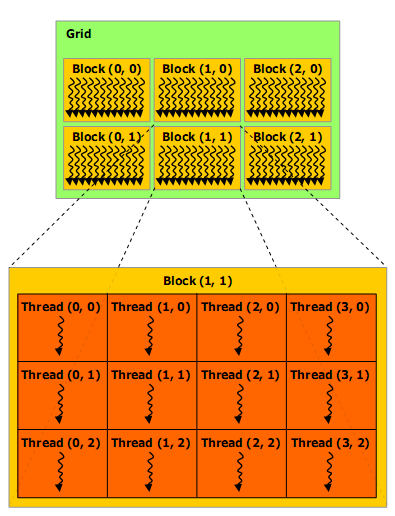
\includegraphics[width=0.4\textwidth]{img/cuda_threads.png}
}
\subfigure[Kernel]{
	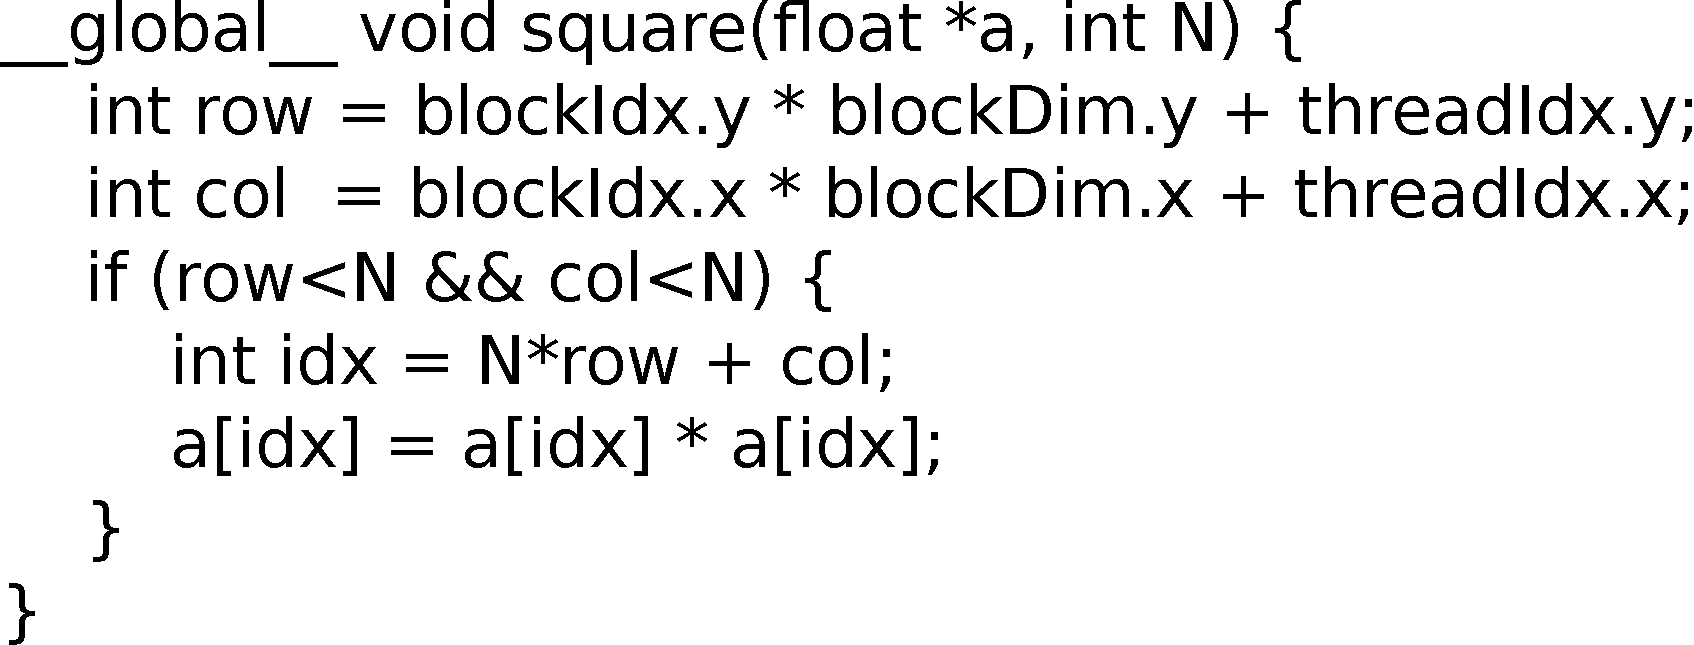
\includegraphics[width=0.5\textwidth]{img/kernel.pdf}
}
\caption{Depicts how GPU threads are grouped into blocks and arranged in a grid. One thread runs a copy of a kernel function, in this example an element-wise matrix square operation.}
\label{fig:gpu_grid}
\end{figure}

\section {Medical ultrasound imaging}\label{sec:ultrasound}
Ultrasound imaging encompasses technology which generates images based on sound whose frequencies we can not hear. For medical ultrasound imaging frequencies above 2 MHz are typically used.

Small section about heart anatomy.

\begin{figure}
\centering
\subfigure{
	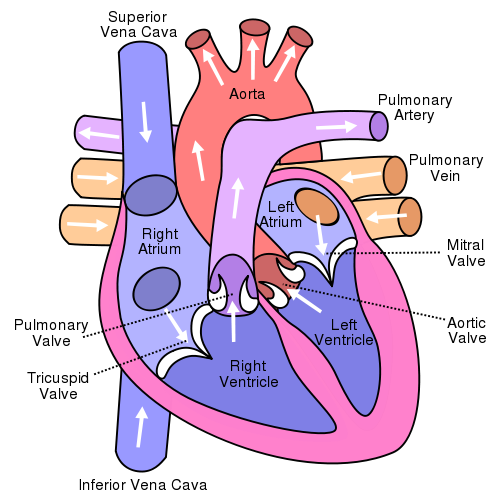
\includegraphics[width=0.47\textwidth]{img/Diagram_of_the_human_heart.png}
}
\subfigure{
	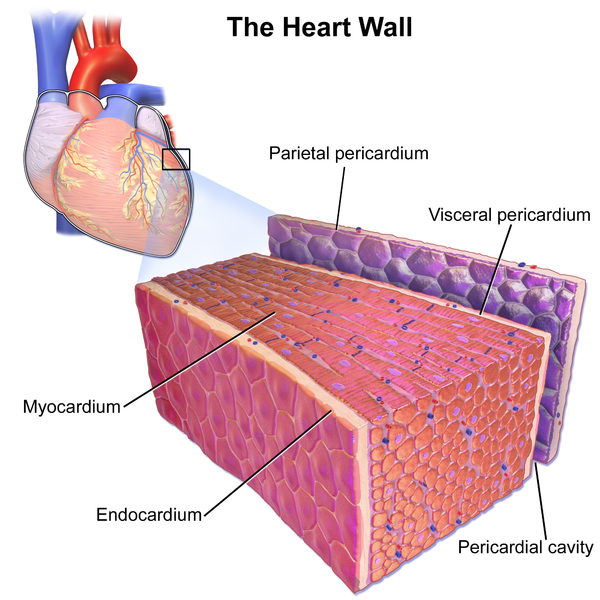
\includegraphics[width=0.47\textwidth]{img/HeartWall.png}
}
\caption{Overview of the human heart. Illustrations from wikipedia.org.}
\label{fig:human_heart}
\end{figure}

Typical probes, scan sequences, resolution and sampling.

Key selling points of ultrasound imaging: cost, safety and real-time user interaction.

One sentence about speckle tracking.
							
\subsection{Basic beamforming}

Delay and sum. Apodization. (See intro to Paper II or III).
Time v.s. phase delays.

\subsection{Adaptive Beamforming}\label{sec:adaptbf}

\begin{figure}[t!]
\subfigure[Delay-and-sum]{
	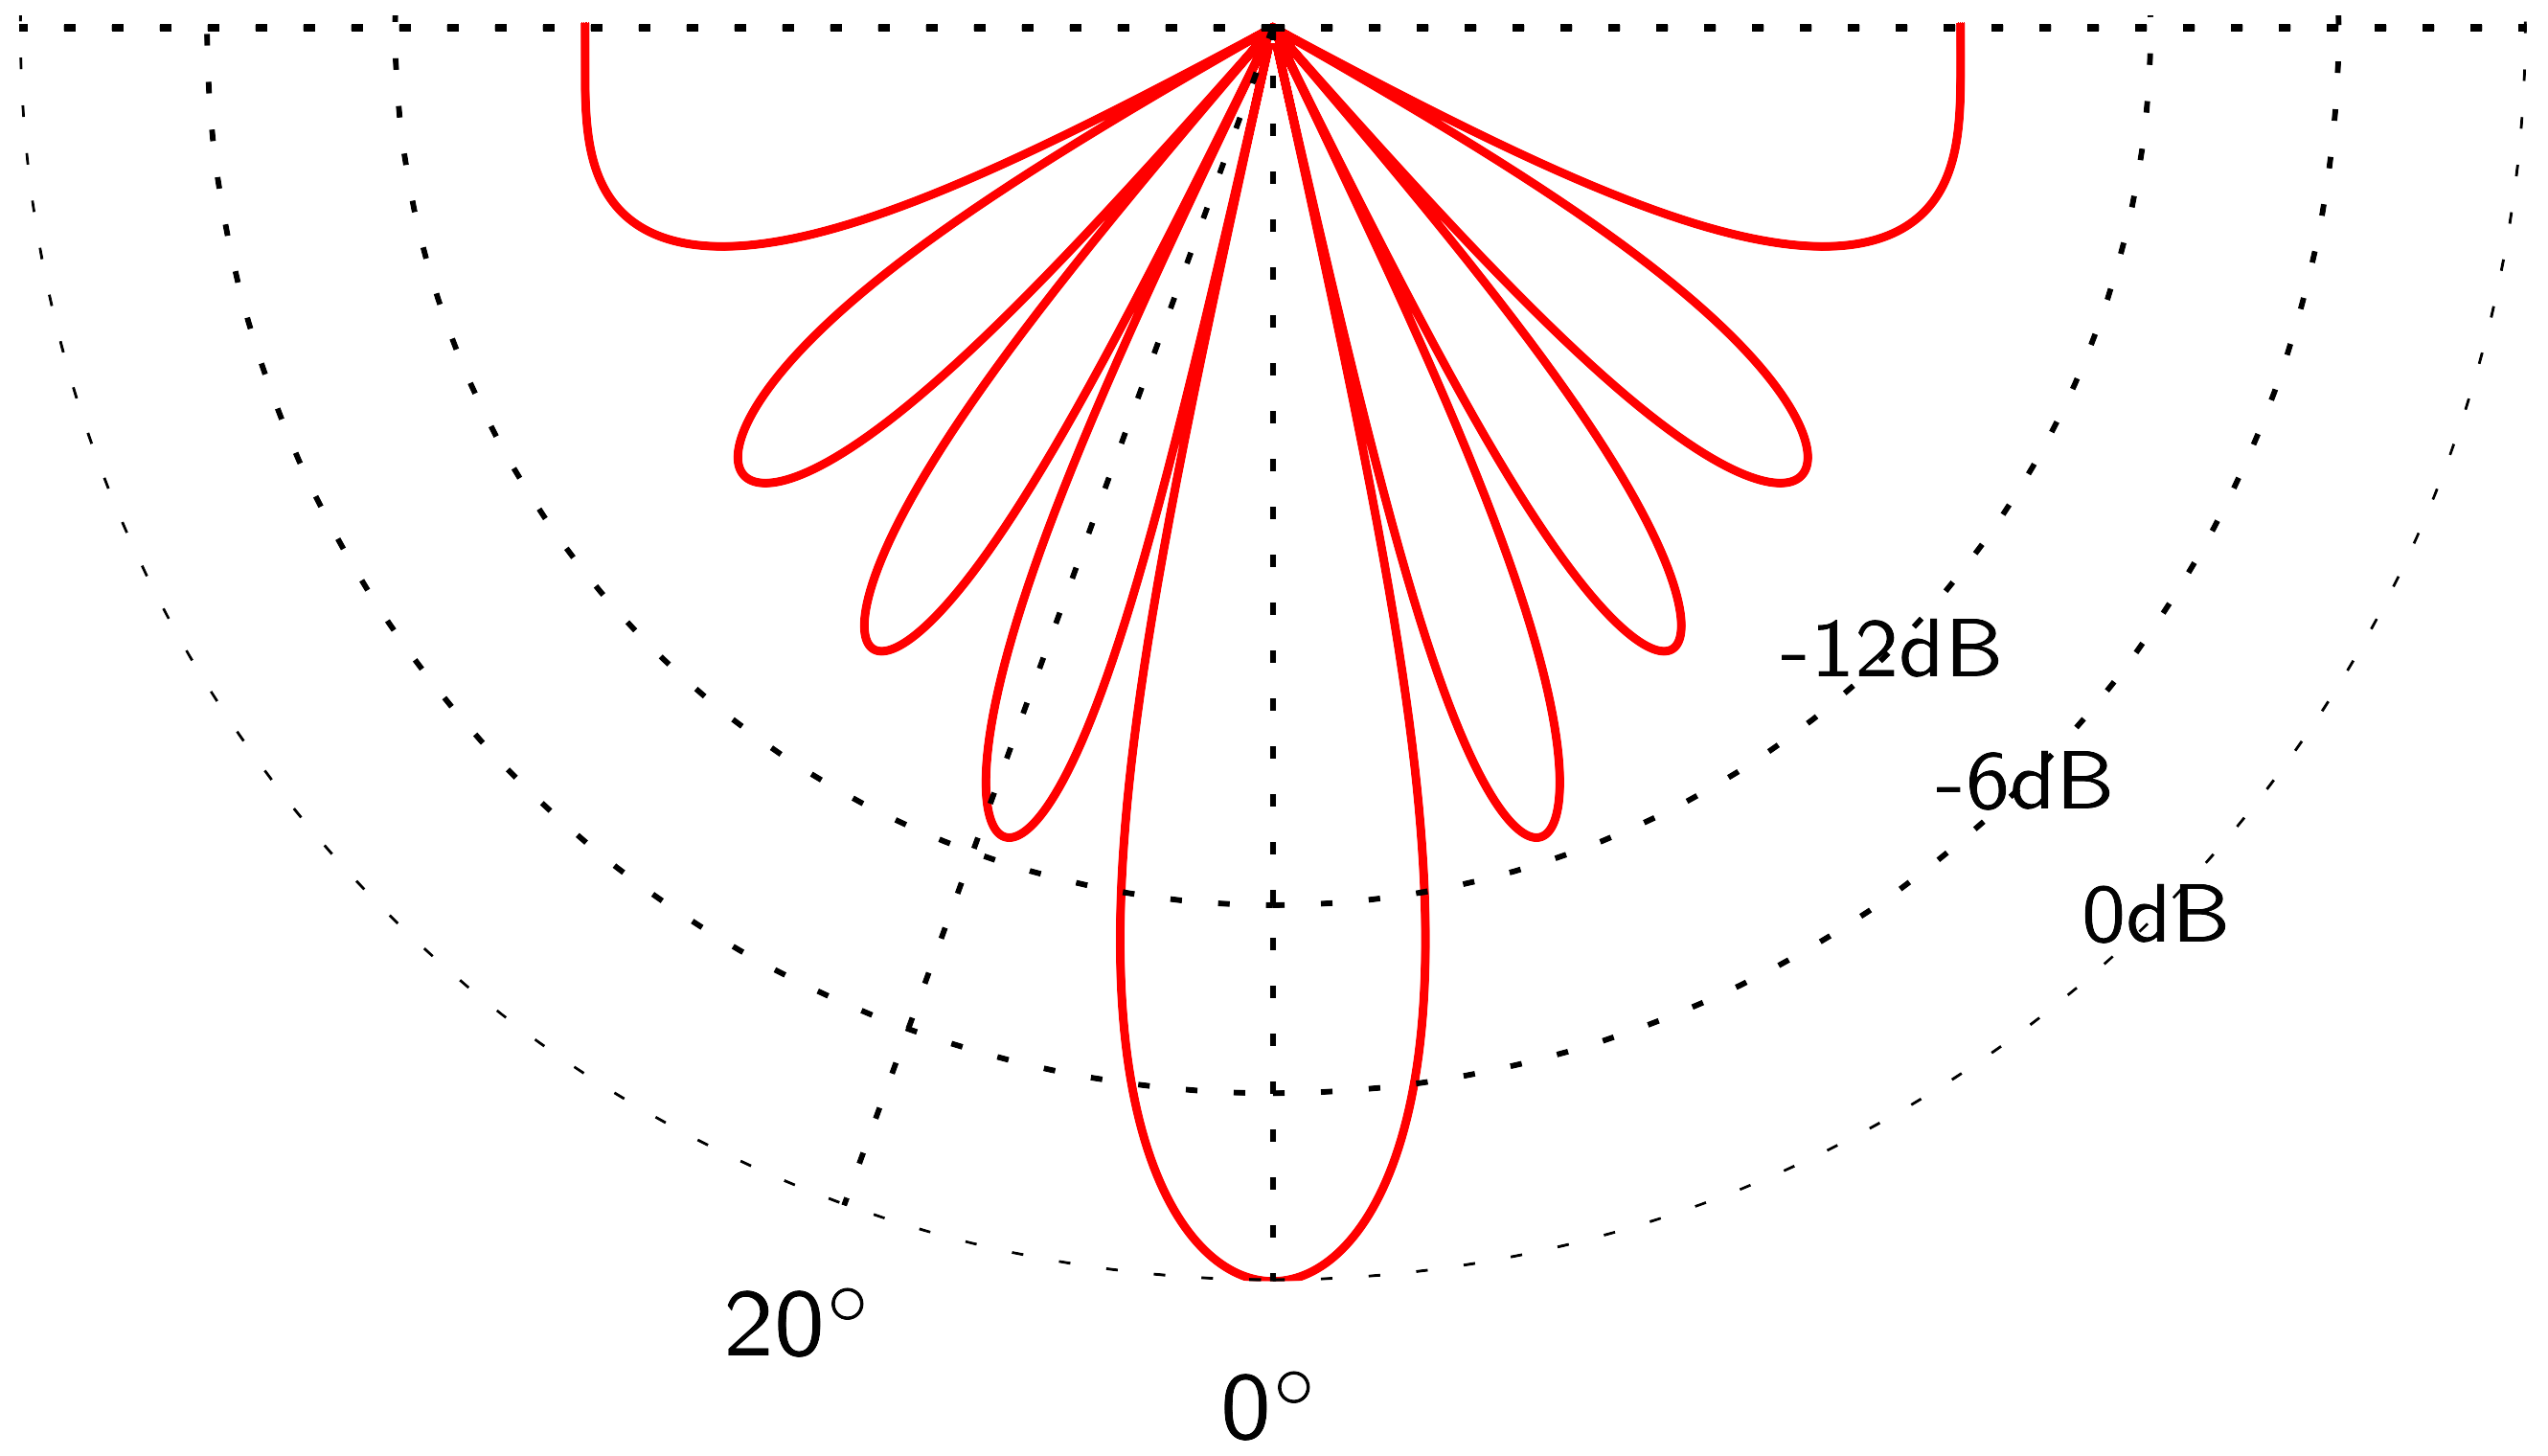
\includegraphics[width=0.47\textwidth]{img/scenario_das_resp2.png}
}
\subfigure[Capon]{
	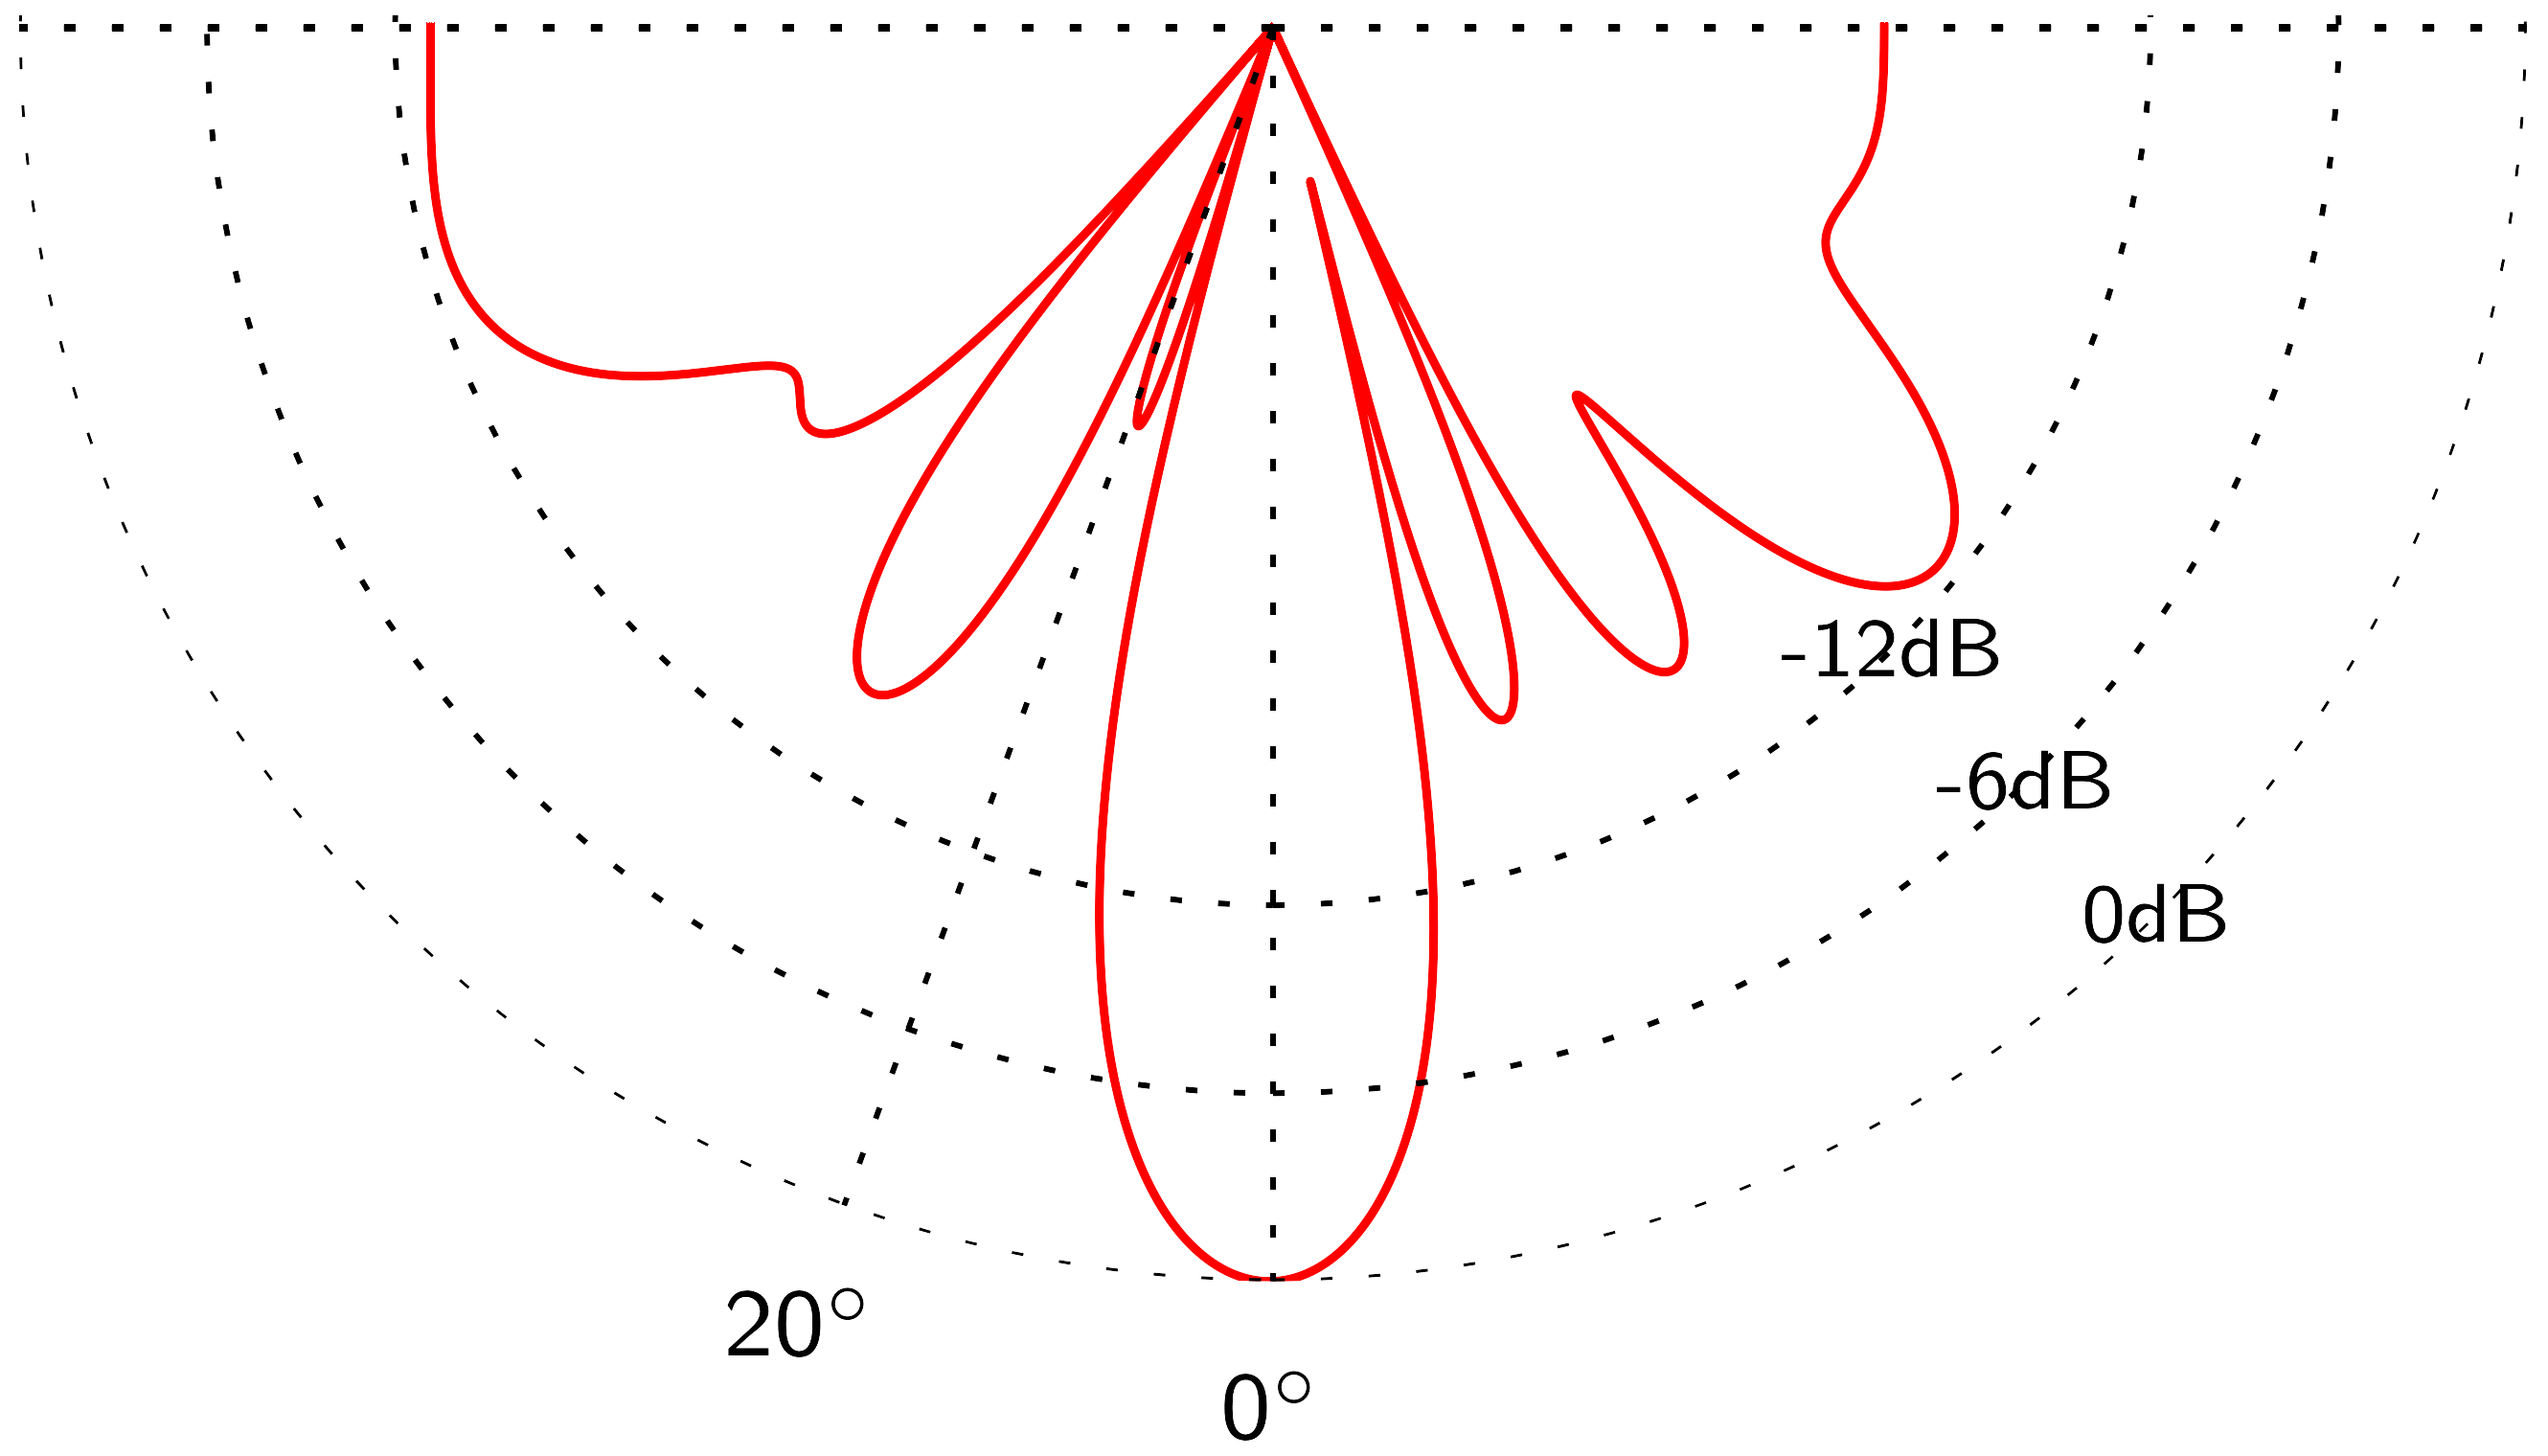
\includegraphics[width=0.47\textwidth]{img/scenario_mv_resp2.png}
}
\caption{Array beam pattern with uniform and Capon weights. An interfering source is located at 20 degrees.}
\end{figure}

Capon beamforming\footnote{The name ''Capon beamformer'' is due to work by J. Capon \todo{add citation} on seismic arrays \todo{Move to background.}} or minimum variance beamforming.

Intro to adaptive beamforming. List other variants (LCA, beamspace, Eigen space etc.). 

Beamspace data is typically refers to the polar grid that cardiac ultrasound data is located in prior to scan conversion. In combination with the Capon beamformer, beamspace refers to the K-space representation of the impinging signals (hence the \nom{FFT}{Fast fourier transform} of the channel data). 

Not phase aberration correction.

Add section about the computationally complexity. How many flops are required per rx-beam etc...

Add section about how to present data (max v.s mean etc.)
						
\subsection{Shift invariance}

\section{Volume rendering}\label{sec:volren}

Get section from master theses. Ray casting and opacity functions.

\begin{figure}
\centering
\subfigure[Ray-casting]{
	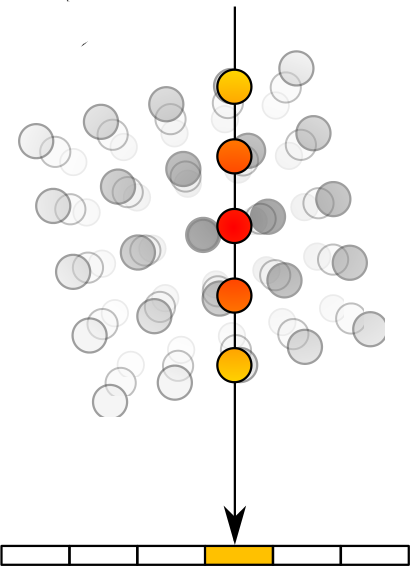
\includegraphics[width=0.4\textwidth]{img/Volumeraycasting.png}
}
\subfigure[Opacity transfer function]{
	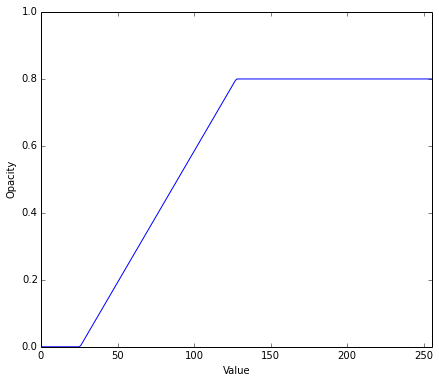
\includegraphics[width=0.5\textwidth]{img/otf.png}
}
\caption{.}
\label{fig:vr}
\end{figure}

\subsection{Adaptive volume rendering}

Visibility driven visualization.

\section{Field simulations}\label{sec:field}

Small chapter about different simulation tools (See hos paper).
			
\endinput
